\documentclass[11pt, a4paper]{article}
\usepackage[a4paper, margin=2.5cm]{geometry}
%% \usepackage{fontspec}
%% \usepackage[english, bidi=basic, provide=*]{babel}
%% \babelprovide[import, onchar=ids fonts]{english}
%% \babelfont{rm}{Noto Sans}
\usepackage{amsmath}
\usepackage{amssymb}
\usepackage{listings}
\usepackage{booktabs}
\usepackage{tabularx}
\usepackage{array}
\usepackage{xcolor}
\usepackage{enumitem}
\usepackage{tikz}
\usetikzlibrary{arrows.meta,matrix, positioning}
\usepackage{graphicx}

\usepackage{hyperref}

\definecolor{accent}{HTML}{1E3A8A}
\definecolor{muted}{HTML}{475569}

\lstset{
    language=Verilog,
    basicstyle=\ttfamily\footnotesize,
    keywordstyle=\color{accent}\bfseries,
    commentstyle=\color{muted}\itshape,
    numbers=left,
    numberstyle=\tiny\color{muted},
    numbersep=6pt,
    frame=single,
    rulecolor=\color{muted},
    breaklines=true,
    columns=fullflexible,
    keepspaces=true,
    showstringspaces=false,
    tabsize=2,
    captionpos=b,
}

\hypersetup{
    colorlinks=true,
    linkcolor=accent,
    urlcolor=accent
}

\setlength{\parindent}{0pt}
\setlength{\parskip}{6pt}

\begin{document}

% ---------------------------------------------------------
% HEADER / TITLE BLOCK
% ---------------------------------------------------------
\begin{center}
    {\LARGE \textbf{\textcolor{accent}{Computer Architecture --- CS 328 (Fall 2026)}}}\\[4pt]
    {\Large \textbf{Complex Engineering Problem}}
\end{center}

\vspace{4pt}
\begin{tabularx}{\textwidth}{@{}X X@{}}
    \toprule
    \textbf{Student 1 Name:} Ukasha & \textbf{Seat No:} CS024115 \\
    \midrule
    \textbf{Student 2 Name:} Abdullah Baig& \textbf{Seat No:} CS-24123 \\
    \bottomrule
\end{tabularx}

\vspace{8pt}
\textbf{Architecture Summary:}

\begin{figure}[htbp]
    \centering

    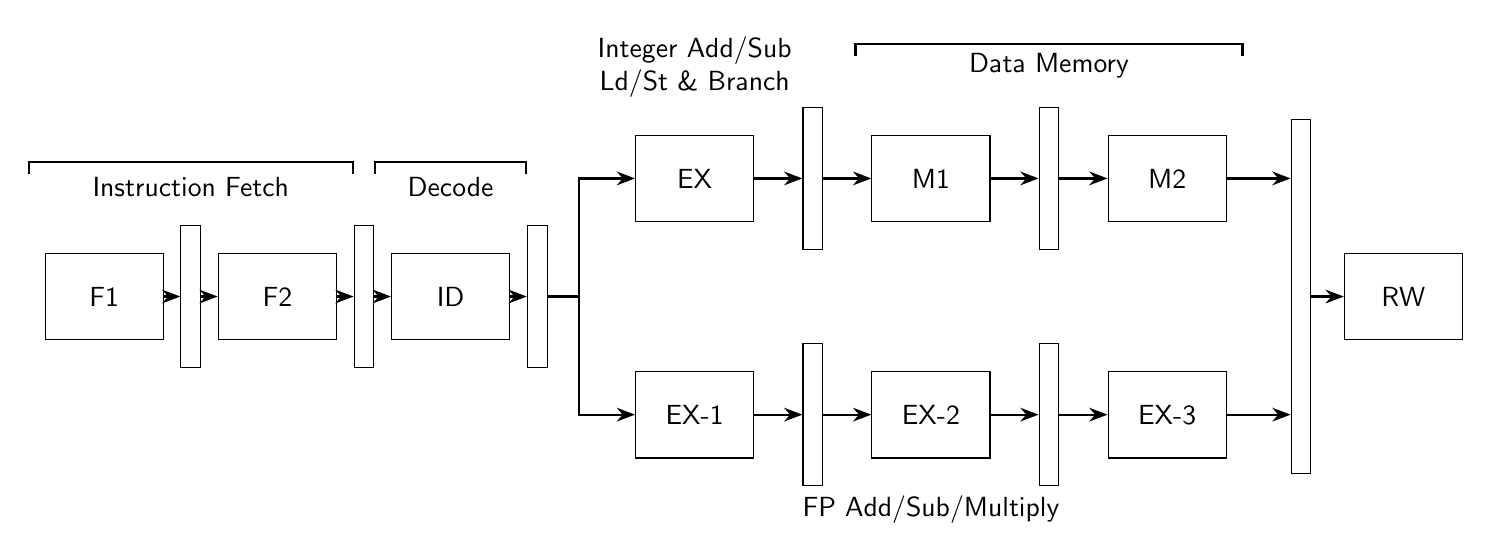
\begin{tikzpicture}[
    font=\sffamily,
    >=Stealth,
    stage/.style={draw, rectangle, minimum width=1.5cm, minimum height=1.1cm, align=center},
    preg/.style={draw, rectangle, minimum width=0.25cm, minimum height=1.8cm, fill=white},
    longpreg/.style={draw, rectangle, minimum width=0.25cm, minimum height=4.5cm, fill=white},
    arr/.style={->, thick}
]

% Nodes - Main sequential path up to ID
\node[stage] (F1) at (0,0) {F1};
\node[preg] (PR1) at (1.1,0) {};
\node[stage] (F2) at (2.2,0) {F2};
\node[preg] (PR2) at (3.3,0) {};
\node[stage] (ID) at (4.4,0) {ID};
\node[preg] (PR3) at (5.5,0) {};

% Top Branch (Integer / Data Memory)
\node[stage] (EX) at (7.5, 1.5) {EX};
\node[preg] (PR4T) at (9.0, 1.5) {};
\node[stage] (M1) at (10.5, 1.5) {M1};
\node[preg] (PR5T) at (12.0, 1.5) {};
\node[stage] (M2) at (13.5, 1.5) {M2};

% Bottom Branch (FP Add/Sub/Multiply)
\node[stage] (EX1) at (7.5, -1.5) {EX-1};
\node[preg] (PR4B) at (9.0, -1.5) {};
\node[stage] (EX2) at (10.5, -1.5) {EX-2};
\node[preg] (PR5B) at (12.0, -1.5) {};
\node[stage] (EX3) at (13.5, -1.5) {EX-3};

% Join Register and RW Stage
\node[longpreg] (PR6) at (15.2, 0) {};
\node[stage] (RW) at (16.5, 0) {RW};

% Horizontal Edges (Fetch / Decode)
\draw[arr] (F1) -- (PR1);
\draw[arr] (PR1) -- (F2);
\draw[arr] (F2) -- (PR2);
\draw[arr] (PR2) -- (ID);
\draw[arr] (ID) -- (PR3);

% Split Edges
\draw[thick] (PR3.east) -- ++(0.4,0) coordinate (split);
\draw[arr] (split) |- (EX.west);
\draw[arr] (split) |- (EX1.west);

% Top Branch Edges
\draw[arr] (EX) -- (PR4T);
\draw[arr] (PR4T) -- (M1);
\draw[arr] (M1) -- (PR5T);
\draw[arr] (PR5T) -- (M2);

% Bottom Branch Edges
\draw[arr] (EX1) -- (PR4B);
\draw[arr] (PR4B) -- (EX2);
\draw[arr] (EX2) -- (PR5B);
\draw[arr] (PR5B) -- (EX3);

% Join Edges
\draw[arr] (M2.east) -- (M2.east -| PR6.west);
\draw[arr] (EX3.east) -- (EX3.east -| PR6.west);
\draw[arr] (PR6.east) -- (RW.west);

% Labels and Brackets
% Instruction Fetch Bracket
\draw[thick] ([xshift=-2mm, yshift=1cm]F1.north west) -- ([xshift=-2mm, yshift=1.15cm]F1.north west) 
          -- ([xshift=2mm, yshift=1.15cm]F2.north east) -- ([xshift=2mm, yshift=1cm]F2.north east);
\node[above, yshift=1.15cm] at (1.1,0) {Instruction Fetch};

% Decode Bracket
\draw[thick] ([xshift=-2mm, yshift=1cm]ID.north west) -- ([xshift=-2mm, yshift=1.15cm]ID.north west) 
          -- ([xshift=2mm, yshift=1.15cm]ID.north east) -- ([xshift=2mm, yshift=1cm]ID.north east);
\node[above, yshift=1.15cm] at (4.4,0) {Decode};

% Data Memory Bracket
\draw[thick] ([xshift=-2mm, yshift=1cm]M1.north west) -- ([xshift=-2mm, yshift=1.15cm]M1.north west) 
          -- ([xshift=2mm, yshift=1.15cm]M2.north east) -- ([xshift=2mm, yshift=1cm]M2.north east);
\node[above, yshift=1.15cm] at (12.0,1.5) {Data Memory};

% Text Labels (No Brackets)
\node[above, align=center, yshift=0.9cm] at (7.5,1.5) {Integer Add/Sub \\ Ld/St \& Branch};
\node[below, yshift=-0.9cm] at (10.5,-1.5) {FP Add/Sub/Multiply};

\end{tikzpicture}

    \caption{Seven-Stage CPU Pipeline Architecture}
    \label{fig:cpu-pipeline}
\end{figure}

\begin{itemize}[noitemsep, topsep=2pt]
    \item \textbf{Integer \& Memory Pipeline:} \texttt{F1} $\rightarrow$ \texttt{F2} $\rightarrow$ \texttt{ID} $\rightarrow$ \texttt{EX} $\rightarrow$ \texttt{M1} $\rightarrow$ \texttt{M2} $\rightarrow$ \texttt{RW} (32 integer registers \texttt{x0}--\texttt{x31}, where \texttt{x0} is hardwired zero).
    \item \textbf{Floating-Point Pipeline:} \texttt{F1} $\rightarrow$ \texttt{F2} $\rightarrow$ \texttt{ID} $\rightarrow$ \texttt{EX-1} $\rightarrow$ \texttt{EX-2} $\rightarrow$ \texttt{EX-3} $\rightarrow$ \texttt{RW} (32 single-precision FP registers \texttt{f0}--\texttt{f31}, where \texttt{f0} is not hardwired zero).
\end{itemize}

\hrule
\vspace{8pt}

% ---------------------------------------------------------
% QUESTION 1
% ---------------------------------------------------------
\section*{\textcolor{accent}{Question 1: Structural Hazard Analysis}}

\subsection*{i. Pipeline Diagram for Unified Memory Structural Hazards}
\textit{Assume a single unified memory (handling both instructions and data) and branch not taken.}
\textit{Data hazards (e.g.\ the \texttt{x10}/\texttt{x24} dependencies) are ignored; only structural hazards are considered.}



\begin{figure}[htbp]
    \centering
    \resizebox{\textwidth}{!}{
    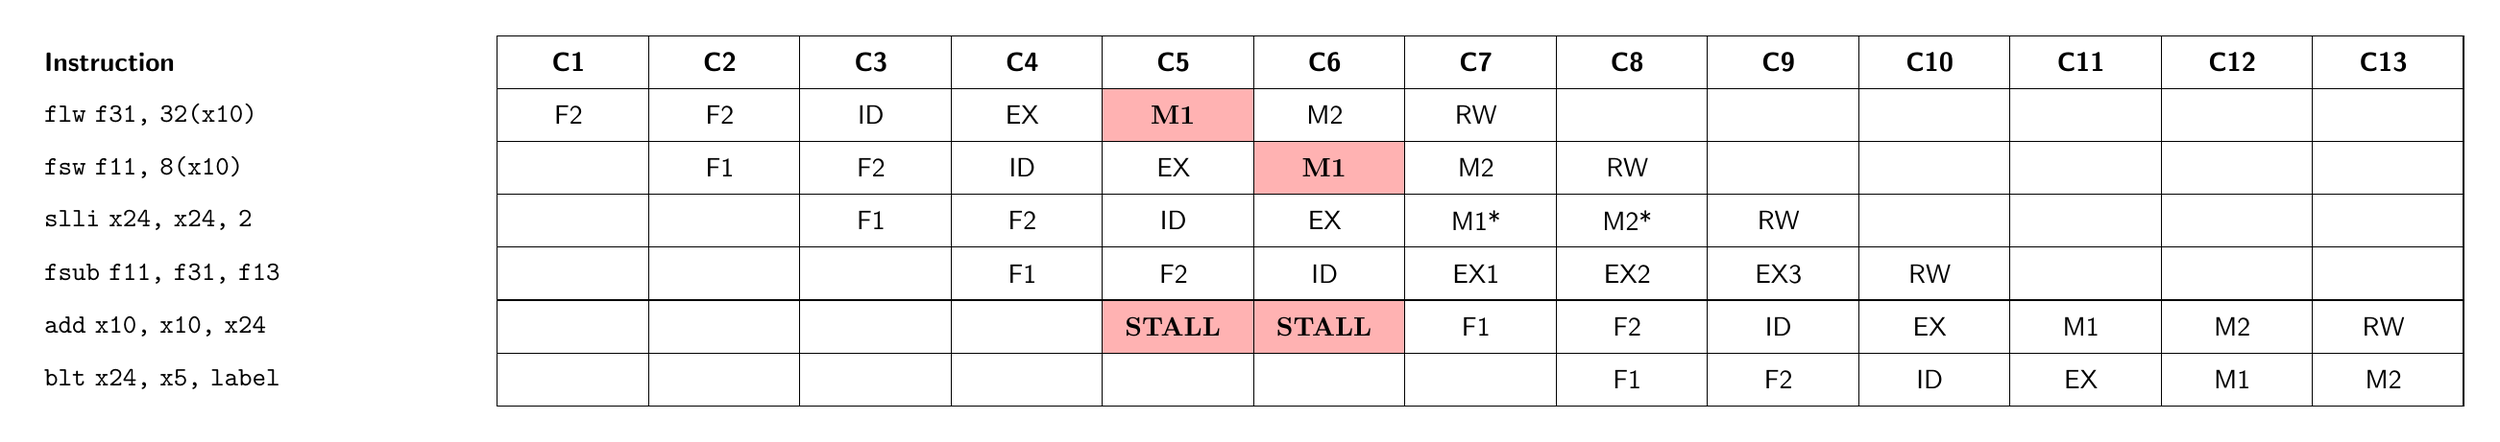
\begin{tikzpicture}[font=\sffamily]

% Pipeline Matrix
\matrix [matrix of nodes,
         nodes={draw, minimum width=2cm, minimum height=0.7cm, anchor=center, align=center},
         column 1/.style={nodes={text width=5.88cm, align=left}}, % Fixes the instruction column width
         column sep=-\pgflinewidth,
         row sep=-\pgflinewidth,
         nodes in empty cells] (pipeline)
{
    |[draw=none]| \textbf{Instruction} & \textbf{C1} & \textbf{C2} & \textbf{C3} & \textbf{C4} & \textbf{C5} & \textbf{C6} & \textbf{C7} & \textbf{C8} & \textbf{C9} & \textbf{C10} & \textbf{C11} & \textbf{C12} & \textbf{C13} \\
    |[draw=none]| \texttt{flw f31, 32(x10)}  & F2 & F2 & ID & EX & |[fill=red!30, font=\bfseries]| M1 & M2 & RW & & & & & & \\
    |[draw=none]| \texttt{fsw f11, 8(x10)}   & & F1 & F2 & ID & EX & |[fill=red!30, font=\bfseries]| M1 & M2 & RW & & & & & \\
    |[draw=none]| \texttt{slli x24, x24, 2}  & & & F1 & F2 & ID & EX & M1* & M2* & RW & & & & \\
    |[draw=none]| \texttt{fsub f11, f31, f13}& & & & F1 & F2 & ID & EX1 & EX2 & EX3 & RW & & & \\
    |[draw=none]| \texttt{add x10, x10, x24} & & & & & |[fill=red!30, font=\bfseries]| STALL & |[fill=red!30, font=\bfseries]| STALL & F1 & F2 & ID & EX & M1 & M2 & RW \\
    |[draw=none]| \texttt{blt x24, x5, label}& & & & & & & & F1 & F2 & ID & EX & M1 & M2 \\
};




\end{tikzpicture}

    }    
    \caption{Structural Hazard}
    \label{fig:q1-pipeline-execution}
    
\end{figure}

\newpage
\textbf{Explanation of Stalls:}
\begin{itemize}[noitemsep, topsep=2pt]
    \item A Structural Hazard happens here because a single pipelined memory is used for both instructions and data, so a conflict occurs whenever an instruction fetch (\texttt{F1}/\texttt{F2}) and a data memory operation (\texttt{M1}/\texttt{M2}) need the same stage of the memory in the same cycle.
    \item In the given code, \texttt{flw} (1st instruction) and \texttt{fsw} (2nd instruction) are the only instructions that actually access data memory in \texttt{M1} and \texttt{M2}. All other instructions only use the CPU's internal pipeline registers during \texttt{M1} and \texttt{M2}.
    \item Since \texttt{M1} is the 5th stage of the pipeline, \texttt{flw} reaches \texttt{M1} in \textbf{Cycle 5} at the exact same time the 5th instruction (\texttt{add x10, x10, x24}) needs to enter \texttt{F1}.
    \item Because both \texttt{M1} and \texttt{F1} use the first stage of the memory, the 5th instruction (\texttt{add}) must stall in \textbf{Cycle 5}.
    \item One stall removes the conflict with \texttt{flw}, but in \textbf{Cycle 6} the 2nd instruction (\texttt{fsw}) enters \texttt{M1}. This causes a second collision with the stalled \texttt{add} instruction trying to enter \texttt{F1}, so \texttt{add} has to stall again in \textbf{Cycle 6} and finally enters \texttt{F1} in \textbf{Cycle 7} (total of \textbf{2 stalls}).
    \item \textbf{Assumption:} Since the unified memory is pipelined into two internal stages (Stage 1 for \texttt{F1}/\texttt{M1} and Stage 2 for \texttt{F2}/\texttt{M2}), Stage 1 and Stage 2 can work in parallel in the same cycle. This means \texttt{fsub} in \texttt{F2} can run alongside \texttt{flw} in \texttt{M1} (Cycle 5), and \texttt{add} in \texttt{F1} can run alongside \texttt{fsw} in \texttt{M2} (Cycle 7) without a second stall per instruction.
    \item After \texttt{fsw} leaves \texttt{M1} at the end of C6, no instruction uses memory stage 1 for data, so no further structural stalls occur. The 7th instruction (\texttt{add x31, x31, x14}) therefore executes normally; its last stages, and the \texttt{RW} of \texttt{blt}, are omitted only because the table stops at C13.
\end{itemize}

\subsection*{ii. Feasibility of Reducing Stalls via Code Reordering}
\begin{itemize}[noitemsep, topsep=2pt]
    \item \textbf{No}, in general, stalls from this structural hazard cannot be reduced by reordering the code.
    \item Every instruction in the program has to be fetched from memory during \texttt{F1} and \texttt{F2}. No matter where we move a \texttt{Load} or \texttt{Store} instruction, when it reaches \texttt{M1} (4 cycles after \texttt{F1}), it will still collide with whichever instruction is four positions later in program order trying to enter \texttt{F1}.
    \item The only rare exception is if we move a memory instruction to the very end of the program (within the last 4 instructions) where there are no more instructions left to fetch when it reaches \texttt{M1}. In normal program execution, there are always instructions following it, so the number of stalls stays the same.
\end{itemize}

\subsection*{iii. Eliminating the Structural Hazard Using Software NOPs}
\begin{itemize}[noitemsep, topsep=2pt]
    \item \textbf{No}, this structural hazard cannot be removed by adding software or compiler \texttt{nop}s.
    \item A software \texttt{nop} (like \texttt{addi x0, x0, 0}) is still a real instruction stored in memory. Even though it does not write to any register or data memory, it still has to be fetched from the memory during \texttt{F1} and \texttt{F2}.
    \item Because fetching a \texttt{nop} in \texttt{F1} still uses the memory in the same cycle that an older memory instruction is in \texttt{M1}, the collision still happens. We need a hardware stall (bubble) that holds the \texttt{PC} and stops the \texttt{F1} fetch for that cycle.
\end{itemize}

\subsection*{iv. Estimated Stall Cycles per 100 Dynamically Executed Instructions}

\begin{center}
\begin{tabular}{@{}l c c c c@{}}
\toprule
\textbf{Category} & \textbf{ALU/Logic} & \textbf{Jump/Branch} & \textbf{Load} & \textbf{Store} \\
\midrule
\textbf{Frequency} & 45\% & 15\% & 25\% & 15\% \\
\bottomrule
\end{tabular}
\end{center}

\textbf{Assumptions:}
\begin{enumerate}[noitemsep, topsep=2pt]
    \item Only structural hazards are considered (no extra stalls or flushes from data hazards or branches). This is a steady-state estimate: it ignores pipeline fill/drain and the last few instructions that have no instruction four positions later.
    \item Only \texttt{Load} and \texttt{Store} instructions use the external memory in \texttt{M1} and \texttt{M2}; \texttt{ALU/Logic} and \texttt{Jump/Branch} do not access data memory.
    \item Because the memory has 2 internal pipeline stages, stalling \texttt{F1} for 1 cycle during \texttt{M1} automatically puts a bubble into \texttt{F2} during \texttt{M2}, allowing the stalled instruction to enter \texttt{F1} while the memory instruction is in \texttt{M2}. Thus, each \texttt{Load} or \texttt{Store} causes \textbf{1 stall cycle}.
    \item All memory accesses are cache hits.
\end{enumerate}

\textbf{Calculation:}
\begin{align*}
    \text{Memory Instructions per 100 Instructions} &= \text{Load (25\%)} + \text{Store (15\%)} = 40\text{ instructions} \\
    \text{Stalls per Memory Instruction} &= 1\text{ cycle} \\
    \text{Total Stall Cycles per 100 Instructions} &= 40 \times 1 = \mathbf{40\text{ stall cycles}}
\end{align*}

\vspace{8pt}
\hrule
\vspace{8pt}

\newpage
% Helper macro using \input
\newcommand{\showdiag}[1]{%
    \begin{center}
        \resizebox{\textwidth}{!}{\input{diagrams/#1.tikz}}
    \end{center}
}
% ---------------------------------------------------------
% QUESTION 2
% ---------------------------------------------------------
\section*{\textcolor{accent}{Question 2: Forwarding Logic Design Trade-offs}}
\subsection*{i. \& ii. Assembly Sequences, Required NOPs, and Pipeline Diagrams}

% --- Pattern 1 ---
\subsubsection*{1. EX to 1st Only (10\%)}
\textbf{4-Instruction Sequence:} \texttt{add x5, x3, x2} $\rightarrow$ \texttt{addi x10, x5, 8} $\rightarrow$ \texttt{add x20, x21, x22} $\rightarrow$ \texttt{sub x23, x24, x25} \\
\textbf{NOPs Required:} 3 \texttt{nop}s inserted after \texttt{add x5, x3, x2}.

\showdiag{dependency-01}

% --- Pattern 2 ---
\subsubsection*{2. MEM to 1st Only (15\%)}
\textbf{4-Instruction Sequence:} \texttt{lw x5, 0(x2)} $\rightarrow$ \texttt{addi x10, x5, 8} $\rightarrow$ \texttt{add x20, x21, x22} $\rightarrow$ \texttt{sub x23, x24, x25} \\
\textbf{NOPs Required:} 3 \texttt{nop}s inserted after \texttt{lw x5, 0(x2)}.

\showdiag{dependency-02}

% --- Pattern 3 ---
\subsubsection*{3. EX to 2nd Only (10\%)}
\textbf{4-Instruction Sequence:} \texttt{add x5, x3, x2} $\rightarrow$ \texttt{add x20, x21, x22} $\rightarrow$ \texttt{addi x10, x5, 8} $\rightarrow$ \texttt{sub x23, x24, x25} \\
\textbf{NOPs Required:} 2 \texttt{nop}s inserted after \texttt{add x20, x21, x22}.

\showdiag{dependency-03}

% --- Pattern 4 ---
\subsubsection*{4. MEM to 2nd Only (10\%)}
\textbf{4-Instruction Sequence:} \texttt{lw x5, 0(x2)} $\rightarrow$ \texttt{add x20, x21, x22} $\rightarrow$ \texttt{addi x10, x5, 8} $\rightarrow$ \texttt{sub x23, x24, x25} \\
\textbf{NOPs Required:} 2 \texttt{nop}s inserted after \texttt{add x20, x21, x22}.

\showdiag{dependency-04}

% --- Pattern 5 ---
\subsubsection*{5. EX to 1st and 2nd (15\%)}
\textbf{4-Instruction Sequence:} \texttt{add x5, x3, x2} $\rightarrow$ \texttt{addi x10, x5, 8} $\rightarrow$ \texttt{sub x11, x5, x4} $\rightarrow$ \texttt{add x20, x21, x22} \\
\textbf{NOPs Required:} 3 \texttt{nop}s inserted after \texttt{add x5, x3, x2}.

\showdiag{dependency-05}

% --- Pattern 6 ---
\subsubsection*{6. EX to 1st and 3rd (5\%)}
\textbf{4-Instruction Sequence:} \texttt{add x5, x3, x2} $\rightarrow$ \texttt{addi x10, x5, 8} $\rightarrow$ \texttt{add x20, x21, x22} $\rightarrow$ \texttt{sub x12, x5, x6} \\
\textbf{NOPs Required:} 3 \texttt{nop}s inserted after \texttt{add x5, x3, x2}.

\showdiag{dependency-06}

% --- Pattern 7 ---
\subsubsection*{7. EX to 2nd and 3rd (5\%)}
\textbf{4-Instruction Sequence:} \texttt{add x5, x3, x2} $\rightarrow$ \texttt{add x20, x21, x22} $\rightarrow$ \texttt{addi x10, x5, 8} $\rightarrow$ \texttt{sub x12, x5, x6} \\
\textbf{NOPs Required:} 2 \texttt{nop}s inserted after \texttt{add x20, x21, x22}.

\showdiag{dependency-07}

% --- Pattern 8 ---
\subsubsection*{8. MEM to 1st and 2nd (10\%)}
\textbf{4-Instruction Sequence:} \texttt{lw x5, 0(x2)} $\rightarrow$ \texttt{addi x10, x5, 8} $\rightarrow$ \texttt{sub x11, x5, x4} $\rightarrow$ \texttt{add x20, x21, x22} \\
\textbf{NOPs Required:} 3 \texttt{nop}s inserted after \texttt{lw x5, 0(x2)}.

\showdiag{dependency-08}

% --- Pattern 09 ---
\subsubsection*{9. MEM to 1st and 3rd (5\%)}
\textbf{4-Instruction Sequence:} \texttt{lw x5, 0(x2)} $\rightarrow$ \texttt{addi x10, x5, 8} $\rightarrow$ \texttt{add x20, x21, x22} $\rightarrow$ \texttt{sub x12, x5, x6} \\
\textbf{NOPs Required:} 3 \texttt{nop}s inserted after \texttt{lw x5, 0(x2)}.

\showdiag{dependency-09}

% --- Pattern 10 ---
\subsubsection*{10. MEM to 2nd and 3rd (8\%)}
\textbf{4-Instruction Sequence:} \texttt{lw x5, 0(x2)} $\rightarrow$ \texttt{add x20, x21, x22} $\rightarrow$ \texttt{addi x10, x5, 8} $\rightarrow$ \texttt{sub x12, x5, x6} \\
\textbf{NOPs Required:} 2 \texttt{nop}s inserted after \texttt{add x20, x21, x22}.

\showdiag{dependency-10}

% --- Pattern 11 ---
\subsubsection*{11. EX to 1st, 2nd and 3rd (5\%)}
\textbf{4-Instruction Sequence:} \texttt{add x5, x3, x2} $\rightarrow$ \texttt{addi x10, x5, 8} $\rightarrow$ \texttt{sub x11, x5, x4} $\rightarrow$ \texttt{add x12, x5, x6} \\
\textbf{NOPs Required:} 3 \texttt{nop}s inserted after \texttt{add x5, x3, x2}.

\showdiag{dependency-11}

% --- Pattern 12 ---
\subsubsection*{12. MEM to 1st, 2nd and 3rd (2\%)}
\textbf{4-Instruction Sequence:} \texttt{lw x5, 0(x2)} $\rightarrow$ \texttt{addi x10, x5, 8} $\rightarrow$ \texttt{sub x11, x5, x4} $\rightarrow$ \texttt{add x12, x5, x6} \\
\textbf{NOPs Required:} 3 \texttt{nop}s inserted after \texttt{lw x5, 0(x2)}.

\showdiag{dependency-12}



\vspace{6pt}
\textbf{General Pattern Observed from NOP Insertion (No Forwarding):}
\begin{itemize}[noitemsep, topsep=2pt]
    \item Without forwarding, it does not matter whether the producer is an \texttt{EX} instruction or a \texttt{MEM} (\texttt{lw}) instruction because both write their final value to the register file at the start of \texttt{RW} (Cycle 7), right before \texttt{ID} reads registers in that same cycle.
    \item \textbf{Whenever the 1st instruction is dependent:} We insert \textbf{3 \texttt{nop}s} right after the producer so that the 1st instruction reaches \texttt{ID} in Cycle 7. Because those 3 \texttt{nop}s also delay the 2nd and 3rd instructions into Cycles 8 and 9, they automatically read the updated register value from the register file without needing any extra \texttt{nop}s.
    \item \textbf{Whenever the 1st instruction is independent and the 2nd is dependent:} The 1st instruction executes normally, and we insert \textbf{2 \texttt{nop}s} before the 2nd instruction so its \texttt{ID} stage lands in Cycle 7. This also shifts the 3rd instruction to Cycle 8, so again no extra \texttt{nop}s are needed for the 3rd instruction.
\end{itemize}

\subsection*{iii. CPI and Stall Percentage with No Forwarding}

\textbf{Grouped Dependency Categories (No Forwarding):}
\begin{itemize}[noitemsep, topsep=2pt]
    \item \textbf{3-Stall Group (1st instruction is dependent):} Includes \texttt{EX to 1st Only} (10\%), \texttt{MEM to 1st Only} (15\%), \texttt{EX to 1st and 2nd} (15\%), \texttt{EX to 1st and 3rd} (5\%), \texttt{MEM to 1st and 2nd} (10\%), \texttt{MEM to 1st and 3rd} (5\%), \texttt{EX to 1st, 2nd and 3rd} (5\%), and \texttt{MEM to 1st, 2nd and 3rd} (2\%). \\
    \textbf{Total Fraction} = $0.10 + 0.15 + 0.15 + 0.05 + 0.10 + 0.05 + 0.05 + 0.02 = \mathbf{67\%}$ ($\text{Stalls} = 3$).
    
    \item \textbf{2-Stall Group (1st independent, 2nd dependent):} Includes \texttt{EX to 2nd Only} (10\%), \texttt{MEM to 2nd Only} (10\%), \texttt{EX to 2nd and 3rd} (5\%), and \texttt{MEM to 2nd and 3rd} (8\%). \\
    \textbf{Total Fraction} = $0.10 + 0.10 + 0.05 + 0.08 = \mathbf{33\%}$ ($\text{Stalls} = 2$).
\end{itemize}

\textbf{Calculation:}
\begin{align*}
    \text{CPI}_{\text{No FW}} &= 1 + \sum \left(\text{Fraction}_i \times \text{Stalls}_i\right) \\
    &= 1 + (0.67 \times 3) + (0.33 \times 2) \\
    &= 1 + 2.01 + 0.66 \\
    &= \mathbf{3.67} \\[6pt]
    \text{Stall Cycle Percentage} &= \left(\frac{\text{CPI}_{\text{No FW}} - 1}{\text{CPI}_{\text{No FW}}}\right) \times 100\% \\
    &= \left(\frac{3.67 - 1}{3.67}\right) \times 100\% \\
    &= \left(\frac{2.67}{3.67}\right) \times 100\% \approx \mathbf{72.75\%}
\end{align*}


\subsection*{iv. CPI and Stall Percentage with Full Forwarding (Including Memory-Stage Forwarding Analysis)}

\textbf{1. Standard Full Forwarding Assumption (All Paths to ALU in EX):}
\begin{itemize}[noitemsep, topsep=2pt]
    \item \textbf{0-Stall Group (50\%):} All \texttt{EX} producer categories use full forwarding (\texttt{EX/M1}, \texttt{M1/M2}, \texttt{M2/RW} to ALU) with 0 stalls.
    \item The table has no ``3rd Only'' row: a 3rd consumer only appears together with a 1st or 2nd consumer, and with full forwarding it is always covered by one of the three paths, so it adds no separate stall.
    \item \textbf{1-Stall Group (18\%):} Includes \texttt{MEM to 2nd Only} (10\%) and \texttt{MEM to 2nd and 3rd} (8\%) waiting 1 cycle to catch \texttt{M2/RW} $\rightarrow$ \texttt{EX} in Cycle 7.
    \item \textbf{2-Stall Group (32\%):} Includes all \texttt{MEM to 1st...} categories (15\% + 10\% + 5\% + 2\%), stalling the 1st instruction for 2 cycles (Cycles 5 and 6) to catch \texttt{M2/RW} $\rightarrow$ \texttt{EX} in Cycle 7.
\end{itemize}

\textbf{Standard Calculation:}
\begin{align*}
    \text{CPI}_{\text{Standard Full FW}} &= 1 + \sum \left(\text{Fraction}_i \times \text{Stalls}_i\right) \\
    &= 1 + (0.32 \times 2) + (0.18 \times 1) \\
    &= 1 + 0.64 + 0.18 = \mathbf{1.82} \\[4pt]
    \text{Stall Cycle Percentage} &= \left(\frac{1.82 - 1}{1.82}\right) \times 100\% \approx \mathbf{45.05\%}
\end{align*}

\vspace{6pt}
\textbf{Architectural extension (not counted in the CPI):} We also considered adding a \emph{second} forwarding unit dedicated to the \texttt{M1} memory stage, so that a load result can bypass directly into a dependent store's data input (or a memory-address calculation) in \texttt{M1}, without waiting for \texttt{EX}. This only helps load-to-store pairs, and the dependency mix in this question does not distinguish store-data consumers from ALU consumers; we treat all \texttt{MEM} consumers as ALU operands. We therefore mention it as an architectural option but claim no CPI improvement for it, and it is not used in the calculations or the recommendation.

\subsection*{v. Feasibility and Disadvantages of Full ALU Forwarding}

\begin{itemize}[noitemsep, topsep=2pt]
    \item \textbf{Feasibility:} Yes, implementing full ALU forwarding is feasible and gives the fastest actual execution time because it drops the CPI from $3.67$ down to $1.82$.
    \item \textbf{Disadvantages:}
        \begin{enumerate}[noitemsep, topsep=1pt]
            \item \textbf{Clock Cycle Time Penalty ($160\text{ ps} \rightarrow 200\text{ ps}$):} Without forwarding (or with only 1 path), the slowest stage in the pipeline is memory (\texttt{M1}/\texttt{M2}) at $160\text{ ps}$. Adding 2 paths stretches \texttt{EX} to $180\text{ ps}$, and adding all 3 paths stretches \texttt{EX} to $200\text{ ps}$. This slows down the global clock by $25\%$ for every instruction in the program, even instructions that have no hazards at all.
            \item \textbf{Extra Hardware and Wiring:} We need larger 4-to-1 multiplexers in front of the ALU inputs, long 32-bit wires coming back from three different pipeline registers, and priority logic in the forwarding unit (so if \texttt{EX/M1} and \texttt{M1/M2} both match, the newer value in \texttt{EX/M1} is chosen).
        \end{enumerate}
\end{itemize}

\subsection*{vi. CPI for Each Single-Stage Forwarding Option}

With only one forwarding path active, the \texttt{EX} stage takes $160\text{ ps}$, which matches \texttt{M1} and \texttt{M2}, so the clock cycle stays at $\mathbf{160\text{ ps}}$. There are two ways the Hazard Detection Unit (HDU) can handle instructions whose exact forwarding path is missing. We use \textbf{Assumption A} for all CPI values below and report Assumption B only as a sensitivity check:
\begin{itemize}[noitemsep, topsep=2pt]
    \item \textbf{Assumption A (primary):} If a later path (like \texttt{M1/M2} or \texttt{M2/RW}) exists, an earlier dependent instruction stalls only until the producer reaches that forwarding stage. These are the natural minimal-stall results.
    \item \textbf{Assumption B (sensitivity only):} If the immediate path for an \texttt{EX} producer is missing, it waits until \texttt{RW} (Cycle 7).
\end{itemize}

\textbf{1. Forwarding ONLY from \texttt{EX/M1} to ALU ($T_{\text{clk}} = 160\text{ ps}$):}
\begin{itemize}[noitemsep, topsep=2pt]
    \item \textbf{0 Stalls (10\%):} \texttt{EX to 1st Only} (10\%) uses \texttt{EX/M1} directly.
    \item \textbf{1 Stall (5\%):} \texttt{EX to 1st and 3rd} (5\%) --- the 1st instruction uses \texttt{EX/M1} with 0 stalls, and the 3rd instruction stalls 1 cycle to read from \texttt{RW} in Cycle 7.
    \item \textbf{2 Stalls (53\%):} \texttt{EX to 1st and 2nd} (15\%) and \texttt{EX to 1st, 2nd and 3rd} (5\%) use \texttt{EX/M1} for the 1st instruction, then stall the 2nd instruction for 2 cycles until \texttt{RW} (which also pushes the 3rd instruction into Cycle 8). \texttt{EX to 2nd Only} (10\%), \texttt{EX to 2nd and 3rd} (5\%), \texttt{MEM to 2nd Only} (10\%), and \texttt{MEM to 2nd and 3rd} (8\%) also stall 2 cycles for \texttt{RW}. Total = $15\% + 5\% + 10\% + 5\% + 10\% + 8\% = 53\%$.
    \item \textbf{3 Stalls (32\%):} All \texttt{MEM to 1st...} categories ($15\% + 10\% + 5\% + 2\% = 32\%$) stall 3 cycles for \texttt{RW}.
\end{itemize}
\begin{align*}
    \text{CPI}_{\text{EX/M1}} &= 1 + (0.05 \times 1) + (0.53 \times 2) + (0.32 \times 3) \\
    &= 1 + 0.05 + 1.06 + 0.96 = \mathbf{3.07}
\end{align*}

\textbf{2. Forwarding ONLY from \texttt{M1/M2} to ALU ($T_{\text{clk}} = 160\text{ ps}$):}
\begin{itemize}[noitemsep, topsep=2pt]
    \item \textbf{0 Stalls (10\%):} \texttt{EX to 2nd Only} (10\%) uses \texttt{M1/M2} directly.
    \item \textbf{1 Stall (20\%):} \texttt{EX to 1st Only} (10\%) and \texttt{EX to 1st and 3rd} (5\%) stall the 1st instruction for 1 cycle so it catches \texttt{M1/M2} (which automatically pushes the 3rd instruction to Cycle 7/\texttt{RW}). \texttt{EX to 2nd and 3rd} (5\%) uses \texttt{M1/M2} for the 2nd instruction and stalls the 3rd instruction 1 cycle for \texttt{RW}. Total = $10\% + 5\% + 5\% = 20\%$.
    \item \textbf{2 Stalls (38\%):} \texttt{EX to 1st and 2nd} (15\%) and \texttt{EX to 1st, 2nd and 3rd} (5\%) stall 1 cycle for the 1st instruction to use \texttt{M1/M2}, and 1 more cycle for the 2nd instruction to reach \texttt{RW} (2 stalls total). \texttt{MEM to 2nd Only} (10\%) and \texttt{MEM to 2nd and 3rd} (8\%) wait 2 cycles for \texttt{RW}. Total = $15\% + 5\% + 10\% + 8\% = 38\%$.
    \item \textbf{3 Stalls (32\%):} All \texttt{MEM to 1st...} categories (32\%) wait 3 cycles for \texttt{RW}.
\end{itemize}
\begin{align*}
    \text{CPI}_{\text{M1/M2}} &= 1 + (0.20 \times 1) + (0.38 \times 2) + (0.32 \times 3) = \mathbf{2.92}
\end{align*}

\textbf{3. Forwarding ONLY from \texttt{M2/RW} to ALU ($T_{\text{clk}} = 160\text{ ps}$):}
\begin{itemize}[noitemsep, topsep=2pt]
    \item \textbf{1 Stall (33\%):} All 2nd-instruction dependent categories without the 1st (\texttt{EX to 2nd...} $15\%$ + \texttt{MEM to 2nd...} $18\% = 33\%$) stall 1 cycle to catch \texttt{M2/RW} in Cycle 7 (pushing the 3rd instruction into \texttt{RW} with 0 extra stalls).
    \item \textbf{2 Stalls (67\%):} All 1st-instruction dependent categories (\texttt{EX to 1st...} $35\%$ + \texttt{MEM to 1st...} $32\% = 67\%$) stall 2 cycles to catch \texttt{M2/RW} in Cycle 7 (which pushes the 2nd and 3rd instructions to Cycles 8 and 9 where they read from \texttt{RW} with 0 extra stalls).
\end{itemize}
\begin{align*}
    \text{CPI}_{\text{M2/RW}} &= 1 + (0.33 \times 1) + (0.67 \times 2) = 1 + 0.33 + 1.34 = \mathbf{2.67}
\end{align*}

\vspace{4pt}
\textbf{Sensitivity check (Assumption B):}
\begin{itemize}[noitemsep, topsep=2pt]
    \item \textbf{\texttt{M1/M2}-only:} $1 + (0.10 \times 0) + (0.05 \times 1) + (0.18 \times 2) + (0.67 \times 3) = \mathbf{3.42}$. The 0-stall group is \texttt{EX to 2nd Only} (10\%), 1 stall is \texttt{EX to 2nd and 3rd} (5\%), 2 stalls are the \texttt{MEM to 2nd} categories (10\% + 8\% = 18\%), and 3 stalls are all 1st-dependent categories (67\%).
    \item \textbf{\texttt{M2/RW}-only:} $1 + (0.18 \times 1) + (0.47 \times 2) + (0.35 \times 3) = \mathbf{3.17}$. The 1-stall group is the \texttt{MEM to 2nd} categories (10\% + 8\% = 18\%), 2 stalls are \texttt{EX to 2nd} (15\%) plus \texttt{MEM to 1st} (32\%) $= 47\%$, and 3 stalls are the \texttt{EX to 1st} categories (35\%).
    \item \textbf{\texttt{EX/M1}-only} is unchanged at $3.07$, because with only that path every later consumer already waits for \texttt{RW}.
\end{itemize}
Assumption A remains the primary result and is what the recommendation uses.

\subsection*{vii. Speedup Comparison and Final Recommendation}

To compare the actual execution time per instruction, we multiply $\text{CPI} \times T_{\text{clk}}$ and compare against the No-Forwarding baseline ($\text{Time}_{\text{No FW}} = 3.67 \times 160\text{ ps} = \mathbf{587.2\text{ ps}}$):
\[
    \text{Speedup} = \frac{\text{Execution Time}_{\text{No FW}}}{\text{Execution Time}_{\text{Option}}} = \frac{587.2\text{ ps}}{\text{CPI}_{\text{Option}} \times T_{\text{clk, Option}}}
\]

\begin{center}
\resizebox{\textwidth}{!}{%
\begin{tabular}{@{}l c c c c@{}}
\toprule
\textbf{Forwarding Configuration} & \textbf{Clock ($T_{\text{clk}}$)} & \textbf{CPI (A / B)} & \textbf{Time / Inst (A / B)} & \textbf{Speedup vs. No FW} \\
\midrule
No Forwarding & $160\text{ ps}$ & $3.67$ & $587.2\text{ ps}$ & $\mathbf{1.00\times}$ (Baseline) \\
Only \texttt{EX/M1} $\rightarrow$ \texttt{EX} & $160\text{ ps}$ & $3.07$ & $491.2\text{ ps}$ & $\mathbf{1.20\times}$ \\
Only \texttt{M1/M2} $\rightarrow$ \texttt{EX} & $160\text{ ps}$ & $2.92$ / $3.42$ & $467.2$ / $547.2\text{ ps}$ & $\mathbf{1.26\times}$ / $\mathbf{1.07\times}$ \\
Only \texttt{M2/RW} $\rightarrow$ \texttt{EX} & $160\text{ ps}$ & $2.67$ / $3.17$ & $427.2$ / $507.2\text{ ps}$ & $\mathbf{1.375\times}$ / $\mathbf{1.16\times}$ \\
Full ALU Forwarding (All 3) & $200\text{ ps}$ & $1.82$ & $364.0\text{ ps}$ & $\mathbf{1.61\times}$ \\
\bottomrule
\end{tabular}}
\end{center}

\textbf{Final Recommendation:}
\begin{itemize}[noitemsep, topsep=2pt]
    \item \textbf{Best Overall Performance:} We recommend \textbf{Full Forwarding}. Even though the clock cycle slows down from $160\text{ ps}$ to $200\text{ ps}$, cutting the CPI down to $1.82$ reduces the total time per instruction from $587.2\text{ ps}$ to $364.0\text{ ps}$ (a $\mathbf{1.61\times}$ speedup).
    \item \textbf{Best Single-Path Option (If Clock Must Stay at $160\text{ ps}$):} If hardware budget is tight and we want to keep the $160\text{ ps}$ clock cycle, forwarding \textbf{only from \texttt{M2/RW}} is the best single-path choice ($\text{CPI} = 2.67$, speedup = $\mathbf{1.375\times}$). 
\end{itemize}

\vspace{8pt}
\hrule
\vspace{8pt}

% ---------------------------------------------------------
% QUESTION 3
% ---------------------------------------------------------



\section*{\textcolor{accent}{Question 3: Forwarding Unit Design and Floating-Point Pipeline}}

\subsection*{i. Integer Pipeline Forwarding Unit Conditions (\texttt{EX/M1}, \texttt{M1/M2}, and \texttt{M2/RW} to \texttt{EX})}

\textbf{Assumptions and Logic:}
\begin{itemize}[noitemsep, topsep=2pt]
    \item Stalling is handled separately by the Hazard Detection Unit (HDU), so the forwarding unit equations remain the same regardless of stalls. The forwarding unit only checks if the instruction currently in \texttt{EX} needs a register value held in \texttt{EX/M1}, \texttt{M1/M2}, or \texttt{M2/RW}.
    \item We assume the \texttt{RegWrite}, \texttt{Rd}, and \texttt{MemRead} control fields are carried in the CPU's \texttt{EX/M1} and \texttt{M1/M2} pipeline registers, and that \texttt{RegWrite}, \texttt{Dest}, and \texttt{FPWrite} are carried in \texttt{M2/RW}. Here \texttt{M2/RW} is the shared write-back register introduced in part iii (the same physical register as \texttt{EX3/RW}); an integer write is present only when \texttt{FPWrite == 0}. These are CPU-side pipeline registers, distinct from the memory's internal pipeline registers.
    \item For paths \texttt{EX/M1} and \texttt{M1/M2}, we check that \texttt{MemRead == 0} because a Load instruction (\texttt{lw}) does not have its data ready until the end of \texttt{M2}. In \texttt{M2/RW}, the \texttt{lw} data is ready, so we do not negate \texttt{MemRead} there.
    \item Since integer register \texttt{x0} is hardwired to zero, we must check that the destination register is not \texttt{x0} ($\texttt{Rd} \neq 0$).
    \item \texttt{RegWrite = 1} for both integer and FP writes, so it cannot tell them apart. On the write-back path we therefore also require \texttt{M2/RW.FPWrite == 0}; otherwise an FP write (or \texttt{flw}) with the same register number would wrongly forward into an integer \texttt{Rs}. The \texttt{EX/M1} and \texttt{M1/M2} paths do not need this check: the only FP write that goes through them is \texttt{flw}, and \texttt{MemRead == 0} already blocks it.
    \item \textbf{Priority Rule:} If more than one later stage writes to the same destination register, we must pick the latest (youngest) instruction. Therefore, \texttt{EX/M1} has the highest priority, \texttt{M1/M2} only forwards if \texttt{EX/M1} does not match, and \texttt{M2/RW} only forwards if neither \texttt{EX/M1} nor \texttt{M1/M2} matches.
\end{itemize}

\textbf{1. Forwarding Logic for First ALU Operand (\texttt{Rs1} / \texttt{ForwardA}):}

\textit{Base Match Conditions for \texttt{Rs1}:}
\begin{align*}
    \text{Cond}_{1A} &= (\texttt{EX/M1.RegWrite} == 1) \text{ and } (\texttt{EX/M1.Rd} \neq 0) \\
                     &\quad \text{and } (\texttt{EX/M1.MemRead} == 0) \text{ and } (\texttt{EX/M1.Rd} == \texttt{ID/EX.Rs1}) \\
    \text{Cond}_{2A} &= (\texttt{M1/M2.RegWrite} == 1) \text{ and } (\texttt{M1/M2.Rd} \neq 0) \\
                     &\quad \text{and } (\texttt{M1/M2.MemRead} == 0) \text{ and } (\texttt{M1/M2.Rd} == \texttt{ID/EX.Rs1}) \\
    \text{Cond}_{3A} &= (\texttt{M2/RW.RegWrite} == 1) \text{ and } (\texttt{M2/RW.FPWrite} == 0) \\
                     &\quad \text{and } (\texttt{M2/RW.Dest} \neq 0) \text{ and } (\texttt{M2/RW.Dest} == \texttt{ID/EX.Rs1})
\end{align*}

\textit{Control Signal Equations for \texttt{ForwardA} (with Priority):}
\begin{itemize}[noitemsep, topsep=2pt]
    \item \textbf{Path 1 (\texttt{EX/M1} $\rightarrow$ \texttt{EX}, \texttt{ForwardA = 1}):}
    \[
        \text{Cond}_{1A}
    \]
    \item \textbf{Path 2 (\texttt{M1/M2} $\rightarrow$ \texttt{EX}, \texttt{ForwardA = 2}):}
    \[
        \overline{\text{Cond}_{1A}} \text{ and } \text{Cond}_{2A}
    \]
    \item \textbf{Path 3 (\texttt{M2/RW} $\rightarrow$ \texttt{EX}, \texttt{ForwardA = 3}):}
    \[
        \overline{\text{Cond}_{1A}} \text{ and } \overline{\text{Cond}_{2A}} \text{ and } \text{Cond}_{3A}
    \]
    \item \textbf{No Forwarding (\texttt{ForwardA = 0}):} Otherwise (read \texttt{Rs1} directly from Register File).
\end{itemize}

\vspace{4pt}
\textbf{2. Forwarding Logic for Second ALU Operand (\texttt{Rs2} / \texttt{ForwardB}):}

\textit{Base Match Conditions for \texttt{Rs2}:}
\begin{align*}
    \text{Cond}_{1B} &= (\texttt{EX/M1.RegWrite} == 1) \text{ and } (\texttt{EX/M1.Rd} \neq 0) \\
                     &\quad \text{and } (\texttt{EX/M1.MemRead} == 0) \text{ and } (\texttt{EX/M1.Rd} == \texttt{ID/EX.Rs2}) \\
    \text{Cond}_{2B} &= (\texttt{M1/M2.RegWrite} == 1) \text{ and } (\texttt{M1/M2.Rd} \neq 0) \\
                     &\quad \text{and } (\texttt{M1/M2.MemRead} == 0) \text{ and } (\texttt{M1/M2.Rd} == \texttt{ID/EX.Rs2}) \\
    \text{Cond}_{3B} &= (\texttt{M2/RW.RegWrite} == 1) \text{ and } (\texttt{M2/RW.FPWrite} == 0) \\
                     &\quad \text{and } (\texttt{M2/RW.Dest} \neq 0) \text{ and } (\texttt{M2/RW.Dest} == \texttt{ID/EX.Rs2})
\end{align*}

\textit{Control Signal Equations for \texttt{ForwardB} (with Priority):}
\begin{itemize}[noitemsep, topsep=2pt]
    \item \textbf{Path 1 (\texttt{EX/M1} $\rightarrow$ \texttt{EX}, \texttt{ForwardB = 1}):}
    \[
        \text{Cond}_{1B}
    \]
    \item \textbf{Path 2 (\texttt{M1/M2} $\rightarrow$ \texttt{EX}, \texttt{ForwardB = 2}):}
    \[
        \overline{\text{Cond}_{1B}} \text{ and } \text{Cond}_{2B}
    \]
    \item \textbf{Path 3 (\texttt{M2/RW} $\rightarrow$ \texttt{EX}, \texttt{ForwardB = 3}):}
    \[
        \overline{\text{Cond}_{1B}} \text{ and } \overline{\text{Cond}_{2B}} \text{ and } \text{Cond}_{3B}
    \]
    \item \textbf{No Forwarding (\texttt{ForwardB = 0}):} Otherwise (read \texttt{Rs2} directly from Register File).
\end{itemize}

\vspace{8pt}
\subsection*{ii. Pipeline Execution Diagram and Clock Cycles}

\showdiag{q3-pipeline}

\textbf{Diagram Notes:}
\begin{itemize}[noitemsep, topsep=2pt]
    \item The \texttt{nop}s are integer \texttt{nop}s (\texttt{addi x0, x0, 0}), so they occupy the integer \texttt{EX}/\texttt{M1}/\texttt{M2}/\texttt{RW} path while the floating-point instructions use \texttt{EX1}/\texttt{EX2}/\texttt{EX3}. The highlighted cells show the \texttt{ID} read of \texttt{fsub}/\texttt{fmul} coinciding with the \texttt{RW} write of its producer.
\end{itemize}

\textbf{Total Clock Cycles Required:}
\begin{itemize}[noitemsep, topsep=2pt]
    \item \textbf{With Forwarding Disabled:} 15 clock cycles (three \texttt{nop}s after each of the two dependent FP instructions).
    \item \textbf{Sanity check with forwarding enabled:} 13 clock cycles (two stalls per dependent FP instruction, using the shared write-back register $\rightarrow$ \texttt{EX1} path described in part iii).
\end{itemize}

\vspace{8pt}
\subsection*{iii. Floating-Point Pipeline Forwarding Unit Conditions (Shared Write-Back Register to \texttt{EX1})}

\textbf{Assumptions and Logic:}
\begin{itemize}[noitemsep, topsep=2pt]
    \item Every FP execution instruction goes through \texttt{EX1}, \texttt{EX2} and \texttt{EX3}, and the result is only ready at the end of \texttt{EX3}. So we cannot forward from \texttt{EX1/EX2} or \texttt{EX2/EX3}.
    \item \textbf{One shared write-back register:} The integer and FP paths are both 7 stages, so \texttt{M2} and \texttt{EX3} are the same stage just before \texttt{RW}. Since the machine is single-issue and in-order, only one instruction can be in \texttt{RW} at a time, so we use one physical register \texttt{RW} instead of separate \texttt{M2/RW} and \texttt{EX3/RW}. A 2:1 mux selects the integer result from \texttt{M2} or the FP result from \texttt{EX3}.
    \item \texttt{RW} carries \texttt{RegWrite}, \texttt{Dest} (either \texttt{Rd} or \texttt{Fd}), \texttt{FPWrite} and the write data. \texttt{FPWrite = 1} writes the FP register file and \texttt{FPWrite = 0} writes the integer one. The load-data mux is before \texttt{RW}, so \texttt{RW} does not need a \texttt{MemToReg} field.
    \item \texttt{flw} uses the integer memory path, so its data is ready at the end of \texttt{M2} and also goes through \texttt{RW}. The FP unit therefore has only one data input, \texttt{RW}, and the same path works for both FP ALU results and \texttt{flw}. A dependent FP instruction then stalls 2 cycles instead of 3.
    \item \texttt{f0} is a normal FP register, not hardwired to zero, so there is no $\texttt{Fd} \neq 0$ check.
    \item \textbf{Pending writers:} A younger writer may still be in \texttt{EX2} or \texttt{EX3}, or in the memory stages for \texttt{flw}, so its value is not ready yet. We call this \texttt{PendingA}/\texttt{PendingB}. While it is true, \texttt{RW} holds an older value, so the forward must be blocked and the consumer has to stall. The stall comes from the HDU (Question 4); Pending is here only to keep the forward equation correct.
\end{itemize}

\textbf{Pending-Writer Match Conditions:}
\begin{align*}
    \text{Pending}_A &= (\texttt{EX1/EX2.RegWrite} == 1) \text{ and } (\texttt{EX1/EX2.Fd} == \texttt{ID/EX1.Fs1}) \\
                     &\quad \text{or } (\texttt{EX2/EX3.RegWrite} == 1) \text{ and } (\texttt{EX2/EX3.Fd} == \texttt{ID/EX1.Fs1}) \\
                     &\quad \text{or } (\texttt{EX/M1.MemRead} == 1) \text{ and } (\texttt{EX/M1.FPWrite} == 1) \\
                     &\quad\qquad \text{and } (\texttt{EX/M1.Rd} == \texttt{ID/EX1.Fs1}) \\
                     &\quad \text{or } (\texttt{M1/M2.MemRead} == 1) \text{ and } (\texttt{M1/M2.FPWrite} == 1) \\
                     &\quad\qquad \text{and } (\texttt{M1/M2.Rd} == \texttt{ID/EX1.Fs1}) \\[2pt]
    \text{Pending}_B &= (\texttt{EX1/EX2.RegWrite} == 1) \text{ and } (\texttt{EX1/EX2.Fd} == \texttt{ID/EX1.Fs2}) \\
                     &\quad \text{or } (\texttt{EX2/EX3.RegWrite} == 1) \text{ and } (\texttt{EX2/EX3.Fd} == \texttt{ID/EX1.Fs2}) \\
                     &\quad \text{or } (\texttt{EX/M1.MemRead} == 1) \text{ and } (\texttt{EX/M1.FPWrite} == 1) \\
                     &\quad\qquad \text{and } (\texttt{EX/M1.Rd} == \texttt{ID/EX1.Fs2}) \\
                     &\quad \text{or } (\texttt{M1/M2.MemRead} == 1) \text{ and } (\texttt{M1/M2.FPWrite} == 1) \\
                     &\quad\qquad \text{and } (\texttt{M1/M2.Rd} == \texttt{ID/EX1.Fs2})
\end{align*}

\textbf{1. FP Forwarding Logic for First Operand (\texttt{Fs1} / \texttt{FP\_ForwardA}):}
\begin{itemize}[noitemsep, topsep=2pt]
    \item \textbf{Path 1 (write-back register $\rightarrow$ \texttt{EX1}, \texttt{FP\_ForwardA = 1}):}
    \[
    \begin{aligned}
        &(\texttt{RW.RegWrite} == 1) \text{ and } (\texttt{RW.FPWrite} == 1) \\
        &\quad \text{and } (\texttt{RW.Dest} == \texttt{ID/EX1.Fs1}) \text{ and } \neg\text{Pending}_A
    \end{aligned}
    \]
    \item \textbf{No Forwarding (\texttt{FP\_ForwardA = 0}):} Otherwise the operand is read from the FP register file. If $\text{Pending}_A$ is true, the forward is blocked and the HDU has to hold the consumer (see Question 4).
\end{itemize}

\textbf{2. FP Forwarding Logic for Second Operand (\texttt{Fs2} / \texttt{FP\_ForwardB}):}
\begin{itemize}[noitemsep, topsep=2pt]
    \item \textbf{Path 1 (write-back register $\rightarrow$ \texttt{EX1}, \texttt{FP\_ForwardB = 1}):}
    \[
    \begin{aligned}
        &(\texttt{RW.RegWrite} == 1) \text{ and } (\texttt{RW.FPWrite} == 1) \\
        &\quad \text{and } (\texttt{RW.Dest} == \texttt{ID/EX1.Fs2}) \text{ and } \neg\text{Pending}_B
    \end{aligned}
    \]
    \item \textbf{No Forwarding (\texttt{FP\_ForwardB = 0}):} Otherwise the operand is read from the FP register file. If $\text{Pending}_B$ is true, the forward is blocked and the HDU has to hold the consumer (see Question 4).
\end{itemize}

\vspace{8pt}
\subsection*{iv. Datapath Interface Diagram for Both Forwarding Units}

\showdiag{forwarding_interface}

\textbf{Mux encoding:} For the integer 4:1 muxes, \texttt{00} = \texttt{ID/EX}, \texttt{01} = \texttt{EX/M1}, \texttt{10} = \texttt{M1/M2}, \texttt{11} = \texttt{RW} (the shared write-back register, used only when \texttt{RW.FPWrite = 0}). For the FP 2:1 muxes, \texttt{0} = \texttt{ID/EX1}, \texttt{1} = \texttt{RW}. The write-back register's own 2:1 source mux selects \texttt{0} = \texttt{M2} (integer result or load data) and \texttt{1} = \texttt{EX3} (FP result).

The FP forwarding unit also receives \texttt{PendingA} and \texttt{PendingB} from part iii. These block the write-back forward while a younger FP writer is still in \texttt{EX2}, \texttt{EX3}, or the memory stages, so the consumer does not forward a stale \texttt{RW} value.



\vspace{8pt}
\hrule
\vspace{8pt}

% ---------------------------------------------------------
% QUESTION 4
% ---------------------------------------------------------
\section*{\textcolor{accent}{Question 4: Hazard Detection Unit}}

Full forwarding removes the ordinary ALU--ALU hazards, but it cannot remove two cases. A load produces its data at the end of \texttt{M2}, so the value is only in the shared write-back register \texttt{M2/RW} when the consumer would need it in \texttt{EX}. An FP ALU instruction produces its result at the end of \texttt{EX3}, so its value is also only in \texttt{M2/RW} when the consumer would need it in \texttt{EX1}. In both cases the consumer must be held in \texttt{ID} until the producer reaches \texttt{RW}. The HDU detects these cases in \texttt{ID} and inserts bubbles; it never stalls an instruction that has already entered \texttt{EX} or \texttt{EX1}.

\subsection*{i. Instruction Sequence Requiring a Stall (with Full Forwarding)}

\textbf{Sequence:} \texttt{lw x5, 0(x2)} $\rightarrow$ \texttt{add x6, x5, x1}.

\texttt{add} needs \texttt{x5} in \texttt{EX}. Without a stall it would be in \texttt{EX} in C5, while \texttt{lw} is only in \texttt{M1}; the load data is not ready until \texttt{lw} reaches \texttt{RW} in C7. The HDU therefore holds \texttt{add} in \texttt{ID} for C5 and C6. \texttt{add} enters \texttt{EX} in C7, in the same cycle that \texttt{lw} writes \texttt{x5}, and the \texttt{M2/RW}$\rightarrow$\texttt{EX} forwarding path supplies the value.

\showdiag{q4-load-use}

\textbf{Other unavoidable cases.} The same alignment argument gives the stall counts below. ``Independent'' means an instruction that neither reads nor writes the producer's destination.

\begin{center}
\small
\begin{tabular}{@{}lccc@{}}
\toprule
\textbf{Producer $\rightarrow$ consumer} & \textbf{0 indep.} & \textbf{1 indep.} & \textbf{2 indep.} \\
\midrule
\texttt{lw} $\rightarrow$ integer ALU & 2 & 1 & 0 \\
\texttt{lw} $\rightarrow$ \texttt{sw} (address or store data) & 2 & 1 & 0 \\
\texttt{flw} $\rightarrow$ FP ALU & 2 & 1 & 0 \\
FP ALU $\rightarrow$ FP ALU & 2 & 1 & 0 \\
integer ALU $\rightarrow$ integer ALU & 0 & 0 & 0 \\
\bottomrule
\end{tabular}
\end{center}

The \texttt{lw}$\rightarrow$\texttt{sw} row uses the \texttt{ForwardB} path from \texttt{M2/RW} to \texttt{EX}, that is, the value after the \texttt{MemToReg} mux. With that path, the store data is forwarded exactly like an ALU operand, so the row is 2/1/0. If the design has no store-data path from that write-back value to \texttt{EX} and the store must instead wait for the load to write back and re-read the register file, the row becomes 3/2/1/0 stalls. We use the 2/1/0 result because Question 3's full forwarding already includes the \texttt{M2/RW}$\rightarrow$\texttt{EX} path.

The FP rows have the same shape because the FP result is not available until the end of \texttt{EX3}; only the shared \texttt{RW} value can be forwarded to \texttt{EX1}. Integer ALU results need no stalls at all because they are available at the end of \texttt{EX} and can be forwarded from \texttt{EX/M1}, \texttt{M1/M2}, or \texttt{M2/RW} to \texttt{EX}.

\subsection*{ii. Hazard Detection Unit (HDU) Stall Conditions \& Held Registers}

\textbf{Notation.} The consumer is in \texttt{ID}, so its source registers are the fields of \texttt{IF/ID}. A producer in \texttt{ID/EX} is in \texttt{EX} this cycle, a producer in \texttt{EX/M1} is in \texttt{M1}, a producer in \texttt{ID/EX1} is in \texttt{EX1}, and a producer in \texttt{EX1/EX2} is in \texttt{EX2}. The control unit supplies valid bits $V_1,V_2$ for the integer source ports and $VF_1,VF_2$ for the FP source ports; unused ports are masked. It also supplies \texttt{usesInt} and \texttt{usesFP}, which are both true for \texttt{fsw} because its base register is integer and its store data is FP. We carry \texttt{FPWrite} alongside \texttt{RegWrite}, \texttt{Rd}, and \texttt{MemRead} in \texttt{EX/M1} and \texttt{M1/M2}; this bit lets the HDU distinguish \texttt{lw} from \texttt{flw} and does not change the forwarding equations of Question 3.

\begin{align*}
\text{IntMatch}(D) &= (D=\texttt{IF/ID.Rs1}\land V_1)\lor(D=\texttt{IF/ID.Rs2}\land V_2),\\
\text{FPMatch}(D) &= (D=\texttt{IF/ID.Fs1}\land VF_1)\lor(D=\texttt{IF/ID.Fs2}\land VF_2).
\end{align*}

\textbf{1. Integer load-use hazard:}
\begin{align*}
\text{Stall}_{\text{lw}} &=
\big[\texttt{ID/EX.MemRead}\land\neg\texttt{ID/EX.FPWrite}
\land\texttt{ID/EX.Rd}\neq0\\
&\qquad\land\text{IntMatch}(\texttt{ID/EX.Rd})\big]\\
&\quad\lor\big[\texttt{EX/M1.MemRead}\land\neg\texttt{EX/M1.FPWrite}
\land\texttt{EX/M1.Rd}\neq0\\
&\qquad\land\text{IntMatch}(\texttt{EX/M1.Rd})\big].
\end{align*}

\textbf{2. FP load-use hazard (\texttt{flw}):}
\begin{align*}
\text{Stall}_{\text{flw}} &=
\big[\texttt{ID/EX.MemRead}\land\texttt{ID/EX.FPWrite}
\land\text{FPMatch}(\texttt{ID/EX.Rd})\big]\\
&\quad\lor\big[\texttt{EX/M1.MemRead}\land\texttt{EX/M1.FPWrite}
\land\text{FPMatch}(\texttt{EX/M1.Rd})\big].
\end{align*}
There is no $\texttt{Rd}\neq0$ check here because \texttt{flw} writes an FP register and \texttt{f0} is a normal register.

\textbf{3. FP ALU hazard:}
\begin{align*}
\text{Stall}_{\text{fp}} &=
\big[\texttt{ID/EX1.RegWrite}\land\texttt{ID/EX1.FPWrite}
\land\text{FPMatch}(\texttt{ID/EX1.Fd})\big]\\
&\quad\lor\big[\texttt{EX1/EX2.RegWrite}\land\texttt{EX1/EX2.FPWrite}
\land\text{FPMatch}(\texttt{EX1/EX2.Fd})\big].
\end{align*}

\textbf{4. Combined stall signal and register controls:}
\begin{align*}
\text{Stall} &= (\texttt{usesInt}\land\text{Stall}_{\text{lw}})
\lor\big(\texttt{usesFP}\land(\text{Stall}_{\text{flw}}\lor\text{Stall}_{\text{fp}})\big),\\
\texttt{PCWrite} &= \neg\text{Stall},\\
\texttt{IF/IDWrite} &= \neg\text{Stall},\\
\texttt{ID/EXFlush} &= \text{Stall}\land\texttt{IntPath},\\
\texttt{ID/EX1Flush} &= \text{Stall}\land\texttt{FPPath},\\
\texttt{BufferWrite} &= \text{Stall}\land\neg\texttt{BufferValid},\\
\texttt{BufferRead} &= \texttt{BufferValid}\land\neg\text{Stall}.
\end{align*}
Here \texttt{IntPath} means the consumer will execute through the integer \texttt{EX} path (integer ALU, \texttt{lw}, \texttt{sw}, \texttt{flw}, \texttt{fsw}, or a branch); \texttt{FPPath} means it will execute through \texttt{EX1} (an FP ALU instruction). For \texttt{fsw} both source types are checked, but only \texttt{ID/EXFlush} is asserted because \texttt{fsw} uses the integer memory path. Since a consumer uses exactly one execution path, at most one of the two flush signals is asserted in a cycle, so the HDU inserts at most one bubble per clock cycle. The buffer is written only on the first stall cycle and is drained after the stall, so \texttt{BufferValid} never exceeds one entry.

\textbf{Why no other terms are needed.}
\begin{itemize}[noitemsep, topsep=2pt]
    \item If a load is in \texttt{M1/M2} (that is, in \texttt{M2}), the next cycle it is in \texttt{M2/RW} and the consumer enters \texttt{EX}; the forwarding unit's \texttt{RW} path supplies the data. Therefore \texttt{M1/M2} must not stall.
    \item If an FP result is in \texttt{EX2/EX3} (that is, in \texttt{EX3}), the next cycle it is in \texttt{RW} and the consumer enters \texttt{EX1}; again the \texttt{RW} path is sufficient. Therefore \texttt{EX2/EX3} must not stall.
    \item If the producer is already in \texttt{M2/RW}, the register file write happens at the beginning of the cycle, before the \texttt{ID} read, so the consumer reads the new value directly. It also does not need a stall.
    \item An integer ALU producer needs no term: its result is forwarded from \texttt{EX/M1} when the consumer is immediately after it, from \texttt{M1/M2} with one instruction between, and from \texttt{M2/RW} with two instructions between.
    \item A destination of \texttt{x0} never causes a stall because \texttt{x0} is hardwired to zero. \texttt{f0} is a real destination and is not masked.
\end{itemize}
This also explains why the FP forwarding unit's \texttt{PendingA}/\texttt{PendingB} check from Question 3 is only a safety check: the HDU does not let the consumer enter \texttt{EX1} until the newest matching FP writer is in \texttt{RW}, so the \texttt{RW} value is not stale.

\textbf{Store data.} For \texttt{sw}, \texttt{Rs2} is the store-data operand and is included in $\text{IntMatch}$ through $V_2$. Because \texttt{ForwardB} can select the \texttt{M2/RW} value in \texttt{EX}, an \texttt{lw}$\rightarrow$\texttt{sw} dependency behaves like an ALU consumer: 2 stalls immediately after the load, 1 with one independent instruction, and 0 with two. This is the reason the table above uses 2/1/0 for the store case. For \texttt{fsw}, the integer base register is covered by $\text{Stall}_{\text{lw}}$ and the FP data register by $\text{FPMatch}$; if the FP forwarding unit also drives the store-data mux, the same 2/1/0 rule applies. If it does not, the FP store data must wait for writeback, which adds one stall.

\textbf{CPU pipeline registers during a stall.}
\begin{center}
\footnotesize
\setlength{\tabcolsep}{4pt}
\begin{tabular}{@{}l l >{\raggedright\arraybackslash}p{5.5cm}@{}}
\toprule
\textbf{Register} & \textbf{Action} & \textbf{Reason} \\
\midrule
\texttt{PC} & hold (\texttt{PCWrite = 0}) & keep the \texttt{PC} at C, the address the memory keeps presenting \\
\texttt{IF/ID} & hold (\texttt{IF/IDWrite = 0}) & keep the consumer and its \texttt{IF/ID.PC} in \texttt{ID} \\
\texttt{Fetch buffer} & write once, then hold & save B and B.PC before \texttt{F2} is overwritten by C \\
\texttt{ID/EX} & insert bubble (\texttt{ID/EXFlush = 1}) & clear the control fields of the instruction that would enter \texttt{EX} \\
\texttt{ID/EX1} & insert bubble (\texttt{ID/EX1Flush = 1}) & clear the control fields of the instruction that would enter \texttt{EX1} \\
\texttt{EX/M1}, \texttt{M1/M2}, \texttt{M2/RW} & advance normally & older integer instructions must drain \\
\texttt{EX1/EX2}, \texttt{EX2/EX3} & advance normally & older FP instructions must drain \\
\bottomrule
\end{tabular}
\end{center}

Clearing \texttt{ID/EX} takes effect at the end of the cycle, so it does not disturb the instruction currently in \texttt{EX}: that instruction drives \texttt{EX} for the whole cycle and latches its result into \texttt{EX/M1} at the same clock edge. The clear only removes the control fields of the instruction that would have followed it, which is the consumer that must remain in \texttt{ID}. This is a stall bubble, not a branch flush; the fetch buffer is the only new storage, and it holds B for the duration of the stall.

\textbf{External instruction memory and the single-entry fetch buffer.} The \texttt{F1}/\texttt{F2} registers are internal to the external instruction memory, so the CPU cannot hold them with \texttt{PCWrite}; they are therefore not drawn in Figure iii. The CPU instead keeps its own copy of the address: the PC is clocked through \texttt{F1/PC} and \texttt{F2/PC}, so it arrives in \texttt{IF/ID.PC} together with its instruction. Branch targets are computed from \texttt{IF/ID.PC}, never from the live fetch \texttt{PC}, because the live \texttt{PC} is already ahead of the instruction in \texttt{ID}.

When the HDU detects a stall, the consumer A is in \texttt{IF/ID} and the next instruction B is in \texttt{F2}. At that moment the live \texttt{PC} still holds C's address, the instruction after B. The HDU freezes the \texttt{PC} at C, so the memory keeps presenting C, and only B is about to be overwritten when C moves into \texttt{F2}. A \emph{single-entry} fetch buffer therefore saves B and B's PC. C does not have to be saved because the held \texttt{PC} still points to it; for a longer stall the memory simply keeps presenting C, so the buffer never needs a second entry.

\begin{center}
\footnotesize
\setlength{\tabcolsep}{4pt}
\begin{tabular}{@{}lcccc >{\raggedright\arraybackslash}p{4.2cm}@{}}
\toprule
\textbf{Cycle} & \texttt{IF/ID} & \texttt{F2} & \texttt{PC} & \textbf{Buffer} & \textbf{Action at next edge} \\
\midrule
t   & A & B & C & empty & stall detected; save B and B.PC \\
t+1 & A & C & C & B & C re-presented; stall continues \\
t+2 & A & C & C & B & B enters \texttt{ID}; A enters \texttt{EX}; PC advances to C+4 \\
t+3 & B & C & C+4 & empty & C enters \texttt{ID} \\
t+4 & C & C+4 & C+8 & empty & C+4 enters \texttt{ID} \\
\bottomrule
\end{tabular}
\end{center}

The table lists the state during each cycle; the listed action completes at the end of that cycle. Thus B is saved only once, C is not duplicated, and no instruction is lost or fetched twice; the fetch stream is not restarted. When B drains from the buffer, \texttt{IF/ID.PC} takes the saved B.PC; otherwise it takes \texttt{F2/PC}. The buffer is controlled by
\[
\texttt{BufferWrite} = \texttt{Stall}\land\neg\texttt{BufferValid},
\qquad
\texttt{BufferRead} = \texttt{BufferValid}\land\neg\texttt{Stall},
\]
so it is written on the first stall cycle and read out after the stall. A separate \texttt{BufferFlush} input clears the entry when a branch redirects the fetch stream.

\textbf{Stall bubble versus branch flush.} The \texttt{ID/EXFlush} and \texttt{ID/EX1Flush} signals above only insert a bubble: they clear the control fields of the instruction that would have moved into \texttt{EX} or \texttt{EX1}, while the consumer stays in \texttt{ID}. They do not discard valid work. A branch flush is different: it clears the fetch buffer valid bit (and the younger fetch registers) and loads the \texttt{PC} with the branch target. It is not asserted for a load-use stall.

\subsection*{iii. ID-Stage and Hazard Detection Unit Interface}

\showdiag{hdu-interface}

\textbf{Inputs.}
\begin{itemize}[noitemsep, topsep=2pt]
    \item \texttt{IF/ID.Rs1}, \texttt{IF/ID.Rs2}, \texttt{IF/ID.Fs1}, \texttt{IF/ID.Fs2}: the consumer's source registers, together with the valid bits $V_1,V_2,VF_1,VF_2$ and the decoded \texttt{usesInt}/\texttt{usesFP} flags.
    \item \texttt{IF/ID.PC}: the consumer's own address, carried alongside the instruction through the CPU-side shadow registers \texttt{F1/PC} and \texttt{F2/PC}, or taken from the fetch buffer when B drains. The branch adder uses this saved value for PC-relative targets. The live fetch \texttt{PC} is not used for branch addressing because it is already ahead of the instruction in \texttt{ID}.
    \item \texttt{BufferValid}: the single-entry fetch buffer's valid bit. The HDU uses it to write B only once on the first stall cycle.
    \item \texttt{ID/EX} and \texttt{EX/M1}: \texttt{MemRead}, \texttt{RegWrite}, \texttt{FPWrite}, and \texttt{Rd}. These detect an integer load in \texttt{EX} or \texttt{M1} and an \texttt{flw} in \texttt{EX} or \texttt{M1}.
    \item \texttt{ID/EX1} and \texttt{EX1/EX2}: \texttt{RegWrite}, \texttt{FPWrite}, and \texttt{Fd}. These detect an FP ALU result in \texttt{EX1} or \texttt{EX2}.
    \item \texttt{M1/M2}, \texttt{EX2/EX3}, and \texttt{M2/RW}: the same destination and control fields. They are shown for completeness but deliberately create no stall term: an instruction in \texttt{M2} or \texttt{EX3} reaches \texttt{RW} in the next cycle, so the \texttt{RW} forwarding path is already sufficient.
\end{itemize}

\textbf{Outputs.}
\begin{itemize}[noitemsep, topsep=2pt]
    \item \texttt{PCWrite}: enables the \texttt{PC}; cleared during a stall so the \texttt{PC} stays at C, the address the memory keeps presenting. After the stall it resumes from C and advances to C+4; it is not reloaded from \texttt{IF/ID.PC}.
    \item \texttt{IF/IDWrite}: enables the \texttt{IF/ID} register; cleared during a stall so the consumer stays in \texttt{ID}.
    \item \texttt{ID/EXFlush}: clears the integer \texttt{ID/EX} control fields, inserting a bubble.
    \item \texttt{ID/EX1Flush}: clears the FP \texttt{ID/EX1} control fields, inserting a bubble.
    \item \texttt{BufferWrite}: captures the instruction in \texttt{F2} and its PC on the first stall cycle.
    \item \texttt{BufferRead}: drains the saved instruction and PC into \texttt{IF/ID} after the stall.
    \item \texttt{BufferFlush}: clears the buffer valid bit on a branch redirect; it is not asserted for a load-use stall.
\end{itemize}

\textbf{Timing example (the sequence from part i).} In C4, \texttt{lw} is in \texttt{EX} and \texttt{add} is in \texttt{ID}. The HDU sees \texttt{ID/EX.MemRead = 1}, \texttt{ID/EX.Rd = 5}, and \texttt{IF/ID.Rs1 = 5}, so $\text{Stall}_{\text{lw}}=1$ and \texttt{Stall}=1. It holds \texttt{PC} and \texttt{IF/ID}, writes the \texttt{F2} instruction into the fetch buffer, and clears \texttt{ID/EX}. In C5 the load has moved to \texttt{EX/M1}, so the second bracket of $\text{Stall}_{\text{lw}}$ is true and the stall repeats; the buffer already holds B, so it is not rewritten. In C6 the load is in \texttt{M1/M2} (that is, in \texttt{M2}); no stall term is true, so the buffer drains B into \texttt{ID}, \texttt{add} enters \texttt{EX} in C7, and it receives the \texttt{M2/RW} value through the forwarding unit. The HDU itself is purely combinational; the single-entry fetch buffer is separate storage that the HDU merely controls.

\vspace{8pt}
\hrule
\vspace{8pt}

% ---------------------------------------------------------
% QUESTION 5
% ---------------------------------------------------------
\section*{\textcolor{accent}{Question 5: Control Hazards}}

\subsection*{i. 2-Bit Saturating Counter Branch Predictor Simulation}
\textit{Initial States: $A = 10$ (Weakly Taken), $B = 00$ (Strongly Not Taken), $C = 11$ (Strongly Taken), $D = 01$ (Weakly Not Taken).}

\begin{center}
\small
\setlength{\tabcolsep}{5pt}
\begin{tabular}{@{}l c c c c c c c c c c c@{}}
\toprule
\textbf{Execution} & \textbf{$t+1$} & \textbf{$t+2$} & \textbf{$t+3$} & \textbf{$t+4$} & \textbf{$t+5$} & \textbf{$t+6$} & \textbf{$t+7$} & \textbf{$t+8$} & \textbf{$t+9$} & \textbf{$t+10$} & \textbf{$t+11$} \\
\midrule
\textbf{Branch}        & A  & B  & A  & C  & A  & D  & C  & A  & B  & A  & C  \\
\textbf{Initial State} & 10 & 00 & 11 & 11 & 11 & 01 & 11 & 10 & 00 & 11 & 11 \\
\textbf{Prediction}    & T  & NT & T  & T  & T  & NT & T  & T  & NT & T  & T  \\
\textbf{Outcome}       & T  & NT & T  & T  & NT & NT & T  & T  & NT & NT & NT \\
\textbf{Correct?}      & \checkmark & \checkmark & \checkmark & \checkmark & $\times$ & \checkmark & \checkmark & \checkmark & \checkmark & $\times$ & $\times$ \\
\textbf{Updated State} & 11 & 00 & 11 & 11 & 10 & 00 & 11 & 11 & 00 & 10 & 10 \\
\bottomrule
\end{tabular}
\end{center}

A prediction is taken whenever the counter's most significant bit is 1 (states \texttt{10} and \texttt{11}). A taken branch increments the counter and a not-taken branch decrements it, saturating at \texttt{11} and \texttt{00} respectively.

\subsection*{ii. Total Mispredictions and Misprediction Rate}
\begin{align*}
    \text{Total Mispredictions} &= 3 \\
    \text{Misprediction Rate} &= \frac{\text{Total Mispredictions}}{11} \times 100\% = \frac{3}{11} \times 100\% \approx \mathbf{27.27\%}
\end{align*}

The three mispredictions occur at $t+5$ (branch A was predicted taken but was not taken), at $t+10$ (branch A was predicted taken but was not taken), and at $t+11$ (branch C was predicted taken but was not taken).

\vspace{8pt}
\hrule
\vspace{8pt}

% ---------------------------------------------------------
% QUESTION 6
% ---------------------------------------------------------
\section*{\textcolor{accent}{Question 6: RISC-V Implementation in SystemVerilog}}

\subsection*{Selected Module \& Design Assumptions}
\begin{itemize}[noitemsep, topsep=2pt]
    \item \textbf{Selected Module:} i. RV32I ALU.
    \item \textbf{Inputs:} \texttt{A} and \texttt{B} are 32-bit operands, and \texttt{ALU\_Control} is a 4-bit operation selector.
    \item \textbf{Outputs:} \texttt{Result} is the 32-bit operation result, and \texttt{Zero} is asserted whenever \texttt{Result} is exactly zero.
    \item \textbf{Timing:} The module is purely combinational; it has no clock, reset, or internal state.
    \item \textbf{Supported operations:} \texttt{AND}, \texttt{OR}, \texttt{ADD}, \texttt{SLL}, \texttt{XOR}, \texttt{SUB}, \texttt{SLT}, \texttt{SRL}, \texttt{SRA}, \texttt{SLTU}, and \texttt{PASS\_B}, using the control codes listed in the table below.
    \item \textbf{Shifts:} The shift amount is \texttt{B[4:0]}, matching the RV32I 5-bit \texttt{shamt} field (0--31); higher bits of \texttt{B} are ignored.
    \item \textbf{Signed operations:} \texttt{SLT} and \texttt{SRA} treat \texttt{A} and \texttt{B} as two's-complement signed values, while \texttt{SLTU} and \texttt{SRL} are unsigned.
    \item \textbf{\texttt{PASS\_B}:} Copies \texttt{B} to \texttt{Result}; this is useful for instructions such as \texttt{LUI} or for passing store data / branch targets through the ALU.
    \item \textbf{Unused control codes:} Any code not listed (for example \texttt{0101}) produces \texttt{Result = 0} and therefore \texttt{Zero = 1}.
    \item \textbf{Scope:} Integer overflow and divide-by-zero are not flagged, as RV32I does not trap on them; register \texttt{x0} is kept at zero by the register file, not by the ALU.
\end{itemize}

\begin{center}
\small
\begin{tabular}{@{}l c l@{}}
\toprule
\textbf{Operation} & \textbf{\texttt{ALU\_Control}} & \textbf{Result} \\
\midrule
\texttt{AND}    & \texttt{0000} & \texttt{A \& B} \\
\texttt{OR}     & \texttt{0001} & \texttt{A | B} \\
\texttt{ADD}    & \texttt{0010} & \texttt{A + B} \\
\texttt{SLL}    & \texttt{0011} & \texttt{A << B[4:0]} \\
\texttt{XOR}    & \texttt{0100} & \texttt{A \^{} B} \\
\texttt{SUB}    & \texttt{0110} & \texttt{A - B} \\
\texttt{SLT}    & \texttt{0111} & \texttt{(\$signed(A) < \$signed(B)) ? 1 : 0} \\
\texttt{SRL}    & \texttt{1000} & \texttt{A >> B[4:0]} \\
\texttt{SRA}    & \texttt{1001} & \texttt{\$signed(A) >>> B[4:0]} \\
\texttt{SLTU}   & \texttt{1010} & \texttt{(A < B) ? 1 : 0} \\
\texttt{PASS\_B}& \texttt{1011} & \texttt{B} \\
\bottomrule
\end{tabular}
\end{center}

\subsection*{Testbench Strategy}
The testbench (\texttt{tb\_alu}) instantiates the ALU and checks both \texttt{Result} and \texttt{Zero} after every stimulus. It first applies a directed test for each of the 11 operations using independently computed expected values, so the directed checks do not simply repeat the DUT logic. It then applies seven edge cases: the largest positive addition (\texttt{32'h7FFFFFFF + 1}), \texttt{0 - 1}, a shift amount of 37 (which must use only \texttt{B[4:0] = 5}), an unused control code (\texttt{0101}) that must return zero, plus three more: \texttt{SLL} by 0, \texttt{SRL} by 31, and \texttt{SRA} by 31. It then runs 200 randomized tests, cycling through all 11 operations while driving random 32-bit operands and comparing against the golden model in \texttt{calculate\_expected}. Mismatches print the control code, expected value, and actual value. A final summary reports the total, passed, and failed counts.

\subsection*{Synthesizable SystemVerilog Source}
\lstinputlisting[language=Verilog, caption={RV32I ALU (\texttt{design.sv})}]{design.sv}

\subsection*{Testbench}
\lstinputlisting[language=Verilog, caption={Self-checking ALU testbench (\texttt{testbench.sv})}]{testbench.sv}

\subsection*{Simulation Result}
The simulation output produced by the testbench is shown in Figure~\ref{fig:alu-sim}.

\begin{figure}[htbp]
    \centering
    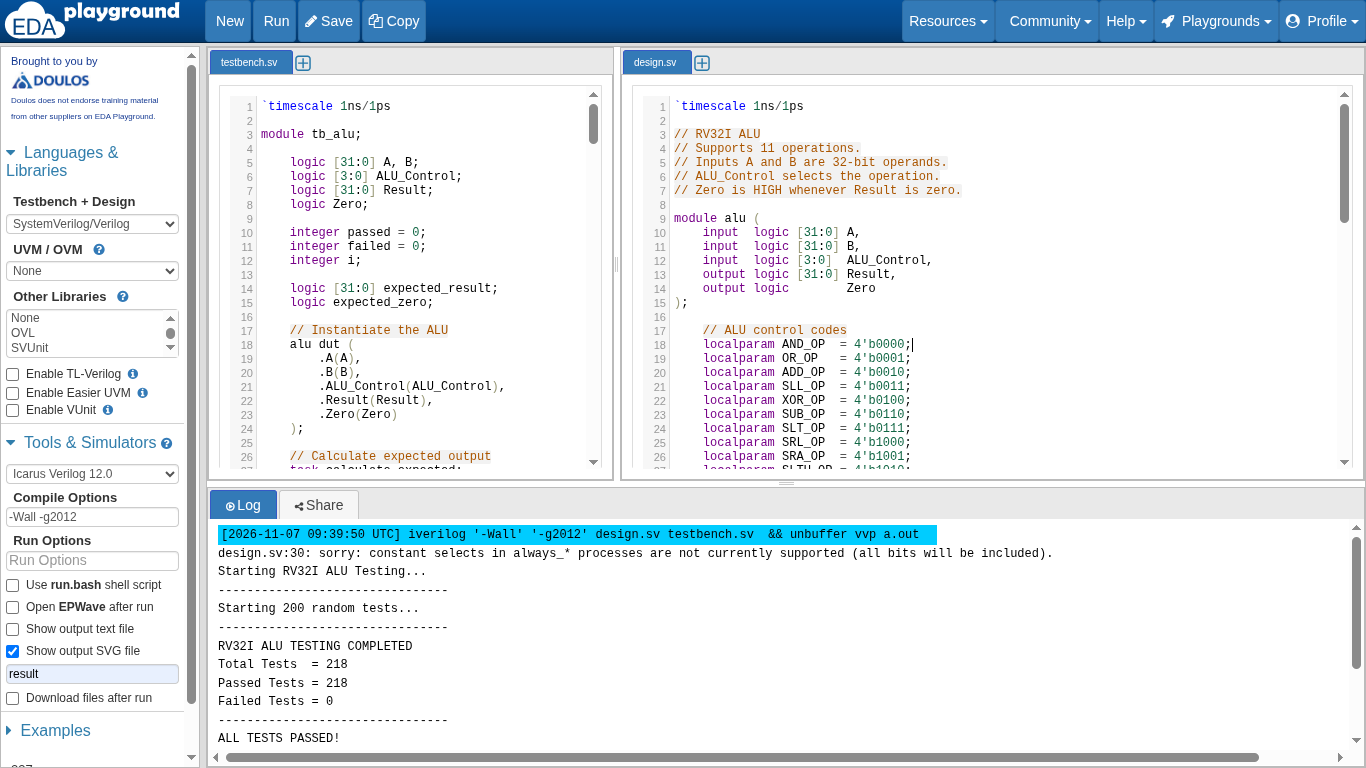
\includegraphics[width=\textwidth]{test-result.png}
    \caption{Simulation output of the RV32I ALU testbench.}
    \label{fig:alu-sim}
\end{figure}

\end{document}
